
\addcontentsline{toc}{chapter}{Analiza istniejącej literatury oraz dotychczasowych badań}
\chapter{Analiza istniejącej literatury oraz dotychczasowych badań}

\section{Can OpenAI Codex and Other Large Language Models Help Us Fix Security Bugs?} \footnotesize\textit{Hammond Pearce, Benjamin Tan, Baleegh Ahmad, Ramesh Karri, Brendan Dolan-Gavitt}
% https://arxiv.org/pdf/2112.02125v1.pdf

\normalsize
\subsection{Metodyka}
W badaniu "Czy OpenAI Codex i inne duże modele językowe mogą pomóc nam naprawić błędy bezpieczeństwa?"\cite{codex-fix-security-bugs} \url{https://arxiv.org/pdf/2112.02125v1.pdf} napisanym przez Hammond'a Pearce'a, Benjamina Tana, Baleegh'a Ahmad, Ramesh'a Karri oraz Brendan'a Dolan-Gavitt, autorzy skupili się na wykorzystaniu dużych modeli językowych (LLM) do naprawy podatności w kodzie w sposób zero-shot. Badanie koncentrowało się na projektowaniu monitów skłaniających LLM do generowania poprawionych wersji niebezpiecznego kodu. Przeprowadzono eksperymenty na szeroką skalę, obejmujące różne komercyjne modele LLM oraz lokalnie wytrenowany model. Problem identyfikacji podatności został rozwiązany przez wykorzystanie istniejących narzędzi statycznej analizy kodu, takich jak CodeQL. Pozwoliło to na izolację problemu badawczego do samego procesu naprawy błędów.

\textbf{Zbadane modele:}
\begin{figure}[H]
    \centering
    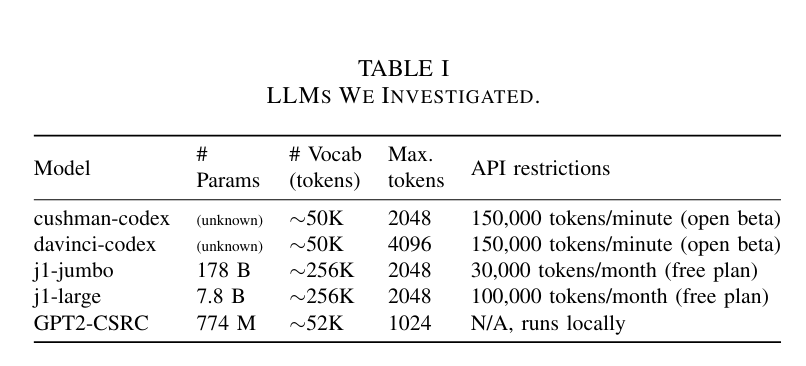
\includegraphics[width=0.8\textwidth]{img/codex-security-models.png}
    \caption{Zastosowane modele językowe w badaniu.}
    \label{fig:codex-fix-security-bugs-models}
\end{figure}

\subsection{Inżynieria zapytań i dane wejściowe}
Kluczową rolę w skuteczności LLM odgrywa inżynieria zapytań. Autorzy zwrócili uwagę na konieczność precyzyjnego sformułowania monitów, aby uzyskać trafne odpowiedzi od modeli. W tym celu wykorzystano różne strategie, takie jak zmiana kontekstu w komentarzach, zmiana temperatury generowania kodu oraz wykorzystanie różnych modeli językowych\ref{fig:codex-fix-security-bugs-models}. Do kreaowania monitów wykorzystano CodeQL\ref{sec:integracja_codeql} do identyfikacji podatności i wstawienia odpowiednich komentarzy w kodzie, aby modele mogły wykonać poprawnie komplecje kodu. 
Użyto dwóch przykładowych programów zawierających podatności CWE-787\footnote{"Out of Bonds" write - zapis poza zakresem} oraz CWE-89\footnote{SQL Injection - wstrzykiwanie złośliwych kwerend SQL} napisanych odpowiednio w językach C i Python do generacji syntetycznych danych testowych, których w sumie powstało 500 wykorzystując modele 'cushman-codex' oraz 'davinci-codex' dla każdej kombinacji 5 różnych temparatur i parametrów 'top\_p'. Użyte zostało także 7 różnych scenariuszy wykonanych ręcznie oraz przykłady z rzeczywistych projektów dostępnych w zbiorze danych \textt{ExtractFix}

\begin{figure}[H]
    \centering
    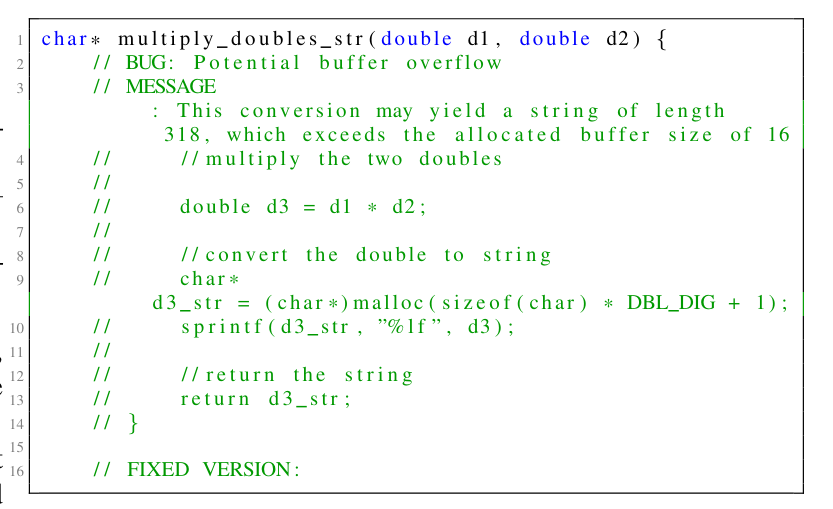
\includegraphics[width=0.8\textwidth]{img/prompt-codex.png}
    \caption{Przykład polecenia w badaniu\cite{codex-fix-security-bugs}.}
    \label{fig:codex-fix-security-bugs-models}
\end{figure}

W badaniu wykorzystano następujące scscenariusze oraz szablony zapytań:
\begin{figure}[H]
    \centering
    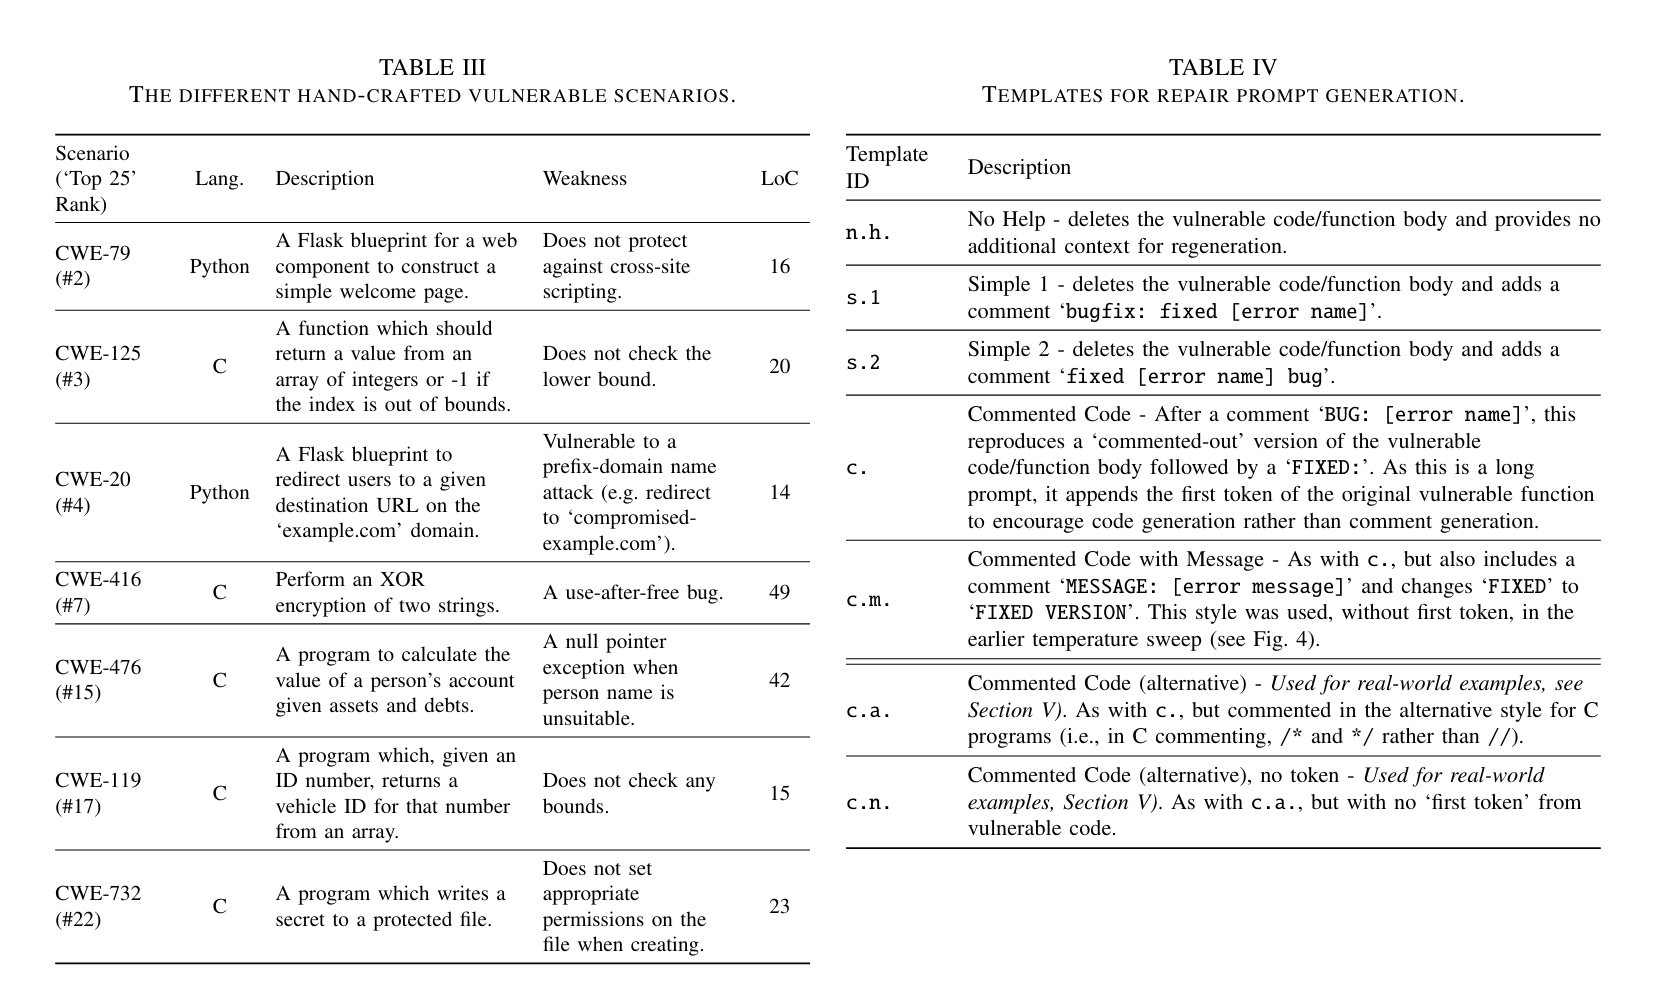
\includegraphics[width=\textwidth]{img/scenarios-codex.png}
    \caption{Scenariusze oraz szablony zapytań obu badań.}
    \label{fig:codex-fix-security-bugs-scenarios}
\end{figure}

\subsection{Wyniki}
Dla każdego z spreparowanych scenariuszy udało się uzyskać funkcjonalne i bezpieczne rozwiązanie w przynajmniej jednej z konfiguracji szablonu zapytania, modelu i parametrów komplecji\footnote{temperatura = \{0.00, 0.25, 0.5, 0.75, 1.00\}, top\_p=1.00}. Odkryto, że różne sposoby formułowania informacji kluczowych w monitach\footnote{ang. prompts} wpływają na wyniki generowane przez modele. Zauważono, że wyższe temperatury generowania kodu przynoszą lepsze wyniki dla niektórych typów podatności, ale gorsze dla innych. 

Tak dobrych wyników niestety nie należy interpretować dosłownie, ponieważ z racji, że badanie przeprowadzono na reprezentatywnej próbie, autorzy nie byli w stanie ręcznie sprawdzać poprawności każdej naprawy i wykorzystali w tym celu istniejące narzędzia statycznej analizy kodu, takie jak CodeQL. W związku z powyższym, aby ocenić rzeczywistą skuteczność LLM w naprawianiu podatności, potrzebne są dalsze badania.

\begin{figure}[ht]
    \centering
    % First image
    \begin{minipage}[b]{0.45\textwidth}
        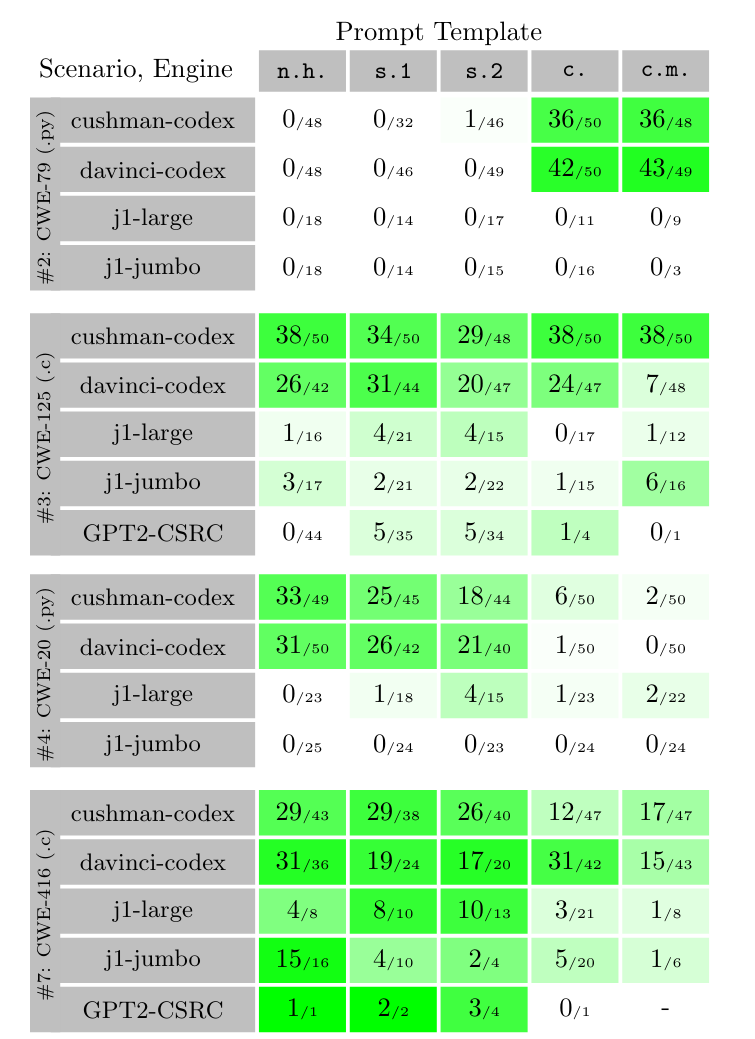
\includegraphics[width=\textwidth]{img/codex-results.png}
        \caption{Wyniki przy użyciu modeli LLM typu black-box do łatania błędów utworzonych syntetycznie. Scenariusze pochodzą z zestawu danych "Diversity of Weakness". Wyniki są sortowane według rankingu "Top 25 CWE" MITRE\dots}
        \label{fig:first_image}
    \end{minipage}
    \hfill
    \begin{minipage}[b]{0.45\textwidth}
        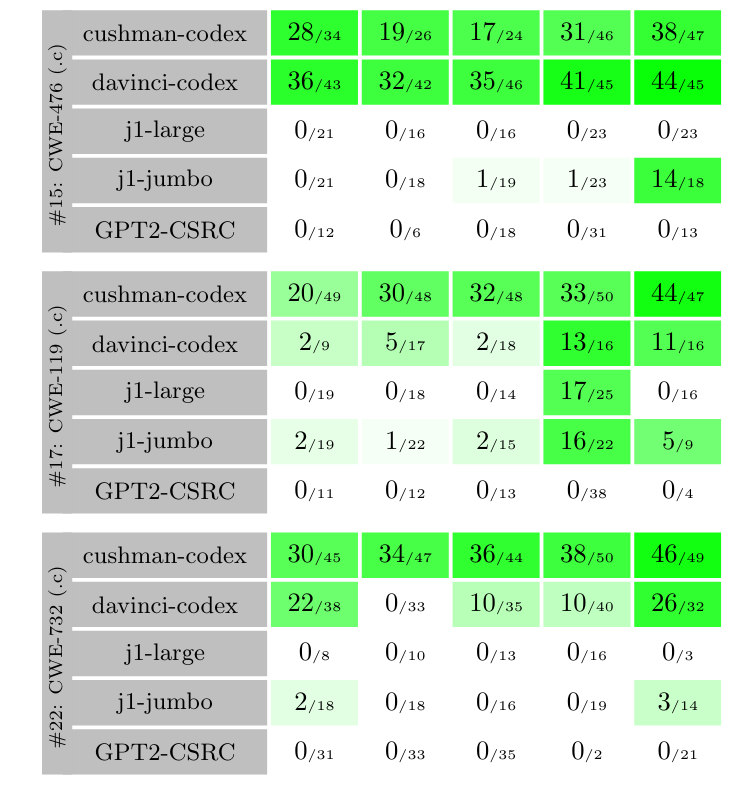
\includegraphics[width=\textwidth]{img/codex-results-2.png}
        \caption{\dots Dla każdej temperatury \{0,00, 0,25, 0,50, 0,75, 1,00\} × top p = \{1,00\} żądano 10 programów (5 dla modeli AI21), dając 50 (25 dla AI21) możliwych programów. Wyniki przedstawiono jako 'bezpieczne i funkcjonalne'/'poprawne (kompilujące się) programy'.}
        \label{fig:second_image}
    \end{minipage}
\end{figure}

\section{Examining Zero-Shot Vulnerability Repair with Large Language Models} \footnotesize\textit{Hammond Pearce, Benjamin Tan, Baleegh Ahmad, Ramesh Karri, Brendan Dolan-Gavitt}
% https://arxiv.org/pdf/2112.02125.pdf

\normalsize
W pracy naukowej pt. "Examining Zero-Shot Vulnerability Repair with Large Language Models"\cite{zero-shot-vuln-repair} \url{https://arxiv.org/pdf/2112.02125.pdf}, autorzy przedłużają swoje badania nad potencjałem wykorzystania Large Language Models (LLM) w kontekście naprawy podatności w kodzie źródłowym. Niniejsze badanie koncentruje się na wyzwaniach związanych z generowaniem funkcjonalnie adekwatnego kodu w realistycznych warunkach aplikacyjnych. Rozszerzając zakres swoich wcześniejszych prac, autorzy skupiają się na bardziej skomplikowanych przypadkach użycia LLM, eksplorując ich zdolność do efektywnego adresowania złożonych problemów związanych z bezpieczeństwem oprogramowania.

Podstawowe pytania badawcze były następujące:
\begin{enumerate}
    \item Czy LLM mogą generować bezpieczny i funkcjonalny kod do naprawy podatności?
    \item Czy zmiana kontekstu w komentarzach wpływa na zdolność LLM do sugerowania poprawek?
    \item Jakie są wyzwania przy używaniu LLM do naprawy podatności w rzeczywistym świecie?
    \item Jak niezawodne są LLM w generowaniu napraw?
\end{enumerate}

\subsection{Metodyka i środki}
Autorzy przeprowadzili eksperymenty na szeroką skalę, wykorzystując różne modele LLM, takie jak OpenAI Codex w różnych wersjach, polycoder, ‘j1-large’ and ‘j1-jumbo’ od AI21 oraz lokalnie wytrenowany model. W celu oceny skuteczności LLM w naprawie podatności, autorzy wykorzystali różne metryki, takie jak skuteczność, precyzja, czułość, F1-score oraz inne miary statystyczne. W badaniu wykorzystano różne techniki inżynierii zapytań, takie jak zmiana kontekstu w komentarzach, zmiana temperatury generowania kodu oraz wykorzystanie różnych modeli językowych. Użyte dane wejściowe\ref{fig:codex-fix-security-bugs-scenarios} zostały wygenerowane syntetycznie, a także pochodziły z rzeczywistych projektów dostępnych w zbiorze danych \textt{ExtractFix}, jak w poprzedniej iteracji badania. W badaniu przeprowadzono też eksperymenty na podatnościach sprzętowych\footnote{ang. hardware}.

\subsection{Wyniki}
Eksperymenty potwierdziły, że choć LLM wykazują potencjał, ich zdolność do generowania funkcjonalnych napraw w rzeczywistych warunkach jest ograniczona. Tak samo jak poprzednio udało się uzyskać przynajmniej jedno rozwiązanie dla każdego scenariusza w przynajmniej jednej konfiguracji. Wyzwania związane z inżynierią promptów i ograniczenia modeli wskazują na potrzebę dalszych badań i rozwoju w tej dziedzinie.

\begin{figure}[ht]
    \centering
    % First image
    \begin{minipage}[b]{0.45\textwidth}
        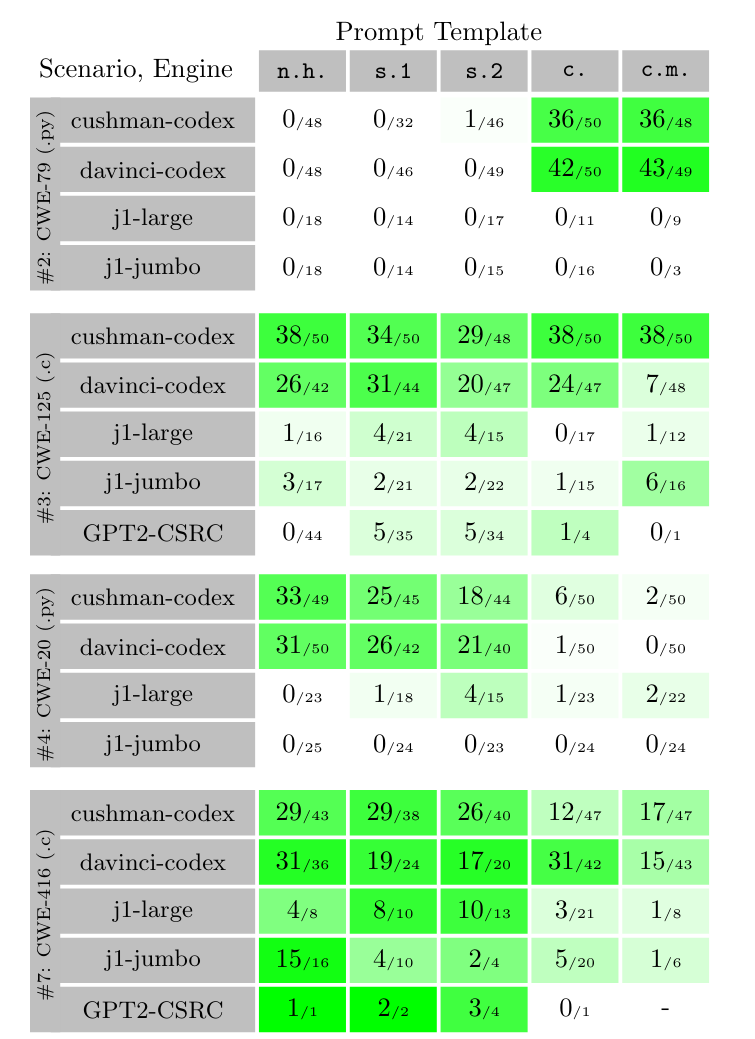
\includegraphics[width=\textwidth]{img/codex-results.png}
        \caption{Wyniki przy użyciu modeli LLM typu black-box do łatania błędów utworzonych syntetycznie. Scenariusze pochodzą z zestawu danych "Diversity of Weakness". Wyniki są sortowane według rankingu "Top 25 CWE" MITRE\dots}
        \label{fig:first_image}
    \end{minipage}
    \hfill
    \begin{minipage}[b]{0.45\textwidth}
        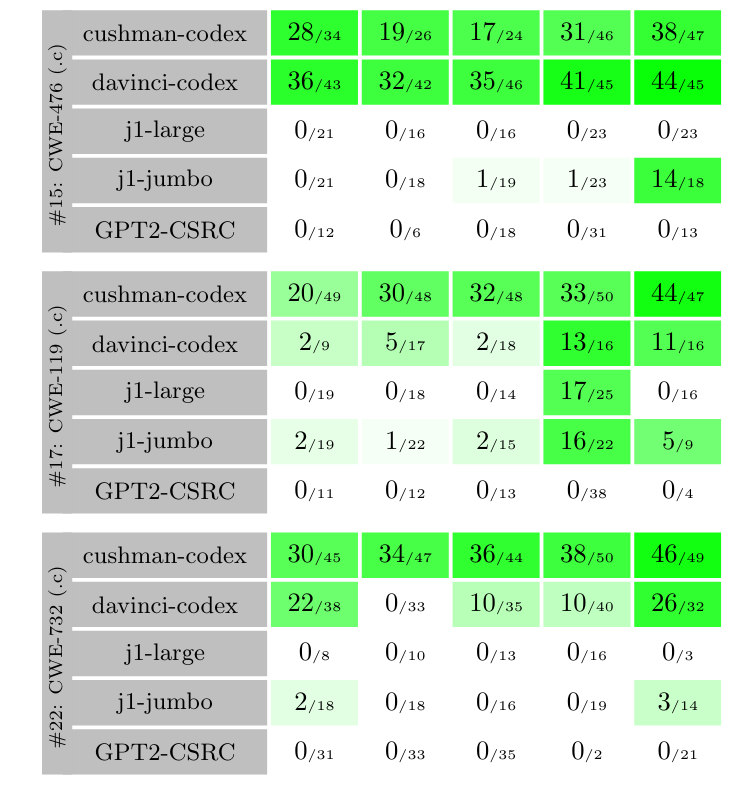
\includegraphics[width=\textwidth]{img/codex-results-2.png}
        \caption{\dots Dla każdej temperatury {0,00, 0,25, 0,50, 0,75, 1,00} × top p {1,00} żądano 10 programów (5 dla modeli AI21), dając 50 (25 dla AI21) możliwych programów. Wyniki przedstawiono jako 'bezpieczne i funkcjonalne'/'poprawne (kompilujące się) programy'.}
        \label{fig:second_image}
    \end{minipage}
\end{figure}


\section{Różnice między obecną pracą a istniejącą literaturą}

W przeciwieństwie do dotychczasowych badań skoncentrowanych głównie na teoretycznym potencjale dużych modeli językowych (LLM) w kontekście zero-shot, niniejsza praca dyplomowa podejmuje kroki w kierunku praktycznego zastosowania tych technologii. 

Główną różnicą jest tutaj zastosowanie metod takich jak Retrieval Augmented Generation (RAG) oraz in-context learning, a także na praktyczne zastosowanie modeli językowych do wykrywania i naprawiania błędów bezpieczeństwa w kodzie. W odróżnieniu od tradycyjnych podejść zero-shot, które polegają na generowaniu odpowiedzi bez uprzedniego pokazania modelowi przykładów do specyficznego zadania, moja praca wykorzystuje RAG i uczenie się w kontekście, aby lepiej dostosować modele do konkretnych scenariuszy związanych z bezpieczeństwem kodu. Te metody wykazują potencjał na uzyskanie precyzyjnej analizy i naprawy błędów w kodzie, a także aktualizują wiedzę modeli o najnowsze podatności na podstawie kontekstu zapytań. 
\begin{itemize}
    \item \textbf{Zastosowanie Metod RAG i In-context Learning:} W odróżnieniu od tradycyjnych podejść zero-shot, które polegają na generowaniu odpowiedzi bez uprzedniego dostosowania modelu do specyficznego zadania, moja praca wykorzystuje RAG i uczenie się w kontekście, aby lepiej dostosować modele do konkretnych scenariuszy związanych z bezpieczeństwem kodu. Te metody pozwalają na bardziej precyzyjną analizę i naprawę błędów w kodzie.
    
    \item \textbf{Praktyczne Zastosowanie Modeli Językowych:} Podczas gdy większość istniejących badań skupia się na badaniu możliwości SI w teorii, ta praca koncentruje się na praktycznym zastosowaniu modeli językowych do wykrywania i naprawiania błędów bezpieczeństwa w kodzie. Przez to podejście, praca ta dostarcza bezpośrednich, aplikatywnych rozwiązań, które mogą być wykorzystane w rzeczywistych środowiskach programistycznych.
\end{itemize}

Takie podejście pozwala nie tylko na zrozumienie teoretycznego potencjału LLM, ale także na ocenę ich praktycznej przydatności w realnych scenariuszach związanych z cyberbezpieczeństwem. Znacząco poszerza to zakres badań w dziedzinie wykorzystania sztucznej inteligencji do poprawy bezpieczeństwa aplikacji, dostarczając nowych perspektyw i rozwiązań.

\chapter{Metodyka rozwiązania}

W niniejszej pracy dyplomowej zastosowano szereg metod i środków, aby zaimplementować narzędzie do statycznej analizy kodu oraz zbadać i ocenić potencjał dużych modeli językowych w kontekście wykrywania i naprawiania błędów bezpieczeństwa w kodzie źródłowym aplikacji.

\begin{table}[H]
    \caption{Metody i środki wykorzystane w projekcie i badaniu.}
    \begin{adjustwidth}{-2cm}{-2cm}  % Zmniejszenie marginesów z obu stron
        \centering
    \begin{tabular}{|>{\bfseries}p{2.7cm}|p{5cm}|>{\bfseries}p{2.5cm}|p{5cm}|}
    \hline
    \multicolumn{4}{|c|}{\textbf{Metody i Środki}} \\
    \hline
    \textbf{Metoda} & \small{Opis} & \textbf{Środek} & \small{Opis} \\
    \hline
    \textbf{Zero-shot learning} & \small{Metoda uczenia maszynowego pozwalająca modelom wykonywać zadania bez wcześniejszego treningu, opierając się na zdolności do rozumienia i generalizacji.} & \textbf{Modele językowe GPT-3.5, GPT-4} & \small{Zaawansowane modele AI OpenAI do generowania tekstu i odpowiadania na zapytania.} \\
    \hline
    \textbf{Prompt engineering} & \small{Projektowanie promptów w celu uzyskania trafnych odpowiedzi od AI.} & \textbf{OpenAI Assistant API} & \small{API umożliwiające integrację modeli językowych w aplikacjach, zaweeirające wiele przydatnych funkcji.\ref{sec:integracja_openai}} \\
    \hline
    \textbf{In-context learning} & \small{Uczenie się i dostosowywanie modeli AI na podstawie informacji zawartych w kontekście zapytań.} & \textbf{Zbiory danych z kodem} & \small{Zestawy danych z przykładami kodu zawierającymi błędy, używane do trenowania narzędzi do wykrywania podatności.} \\
    \hline
    \textbf{Retrieval Augmented Generation} & \small{Technika łącząca generowanie treści z wyszukiwaniem informacji, wspomagana przez OpenAI Assistant API.} & \textbf{Projekty open-source zawierające podatności} & \small{Publiczne projekty zawierające błędy bezpieczeństwa, używane w testowaniu aplikacji oraz ocenie skuteczności LLM.} \\
    \hline
    \textbf{Analiza porównawcza} & \small{Ocena różnych technik lub systemów poprzez porównanie.} & \textbf{Statyczne testy podatności} & \small{Narzędzia analizy statycznej kodu, np. CodeQL.} \\
    \hline
    \textbf{Programowanie obiektowe i funkcyjne} & \small{Dwa paradygmaty programowania, koncentrujące się odpowiednio na obiektach i funkcjach.} & \textbf{Python 3.12} & \small{Najnowsza wersja języka Python z zaawansowanymi funkcjami. Wykorzystywane biblioteki: \texttt{openai, asyncio, tiktoken, scipy, gitpython, csv}} \\
    \hline
 \end{tabular}
\end{adjustwidth}
    \label{tab:methods_tools}
\end{table}
\newpage
Metody i środki te zostały wybrane, aby zapewnić efektywne i wszechstronne podejście do analizy i naprawy kodu. Generacja wspomagana pobieraniem danych (RAG ang. Retrieval Augmented Generation) oraz uczenie się w kontekście(in-context learning) umożliwiają efektywną analizę i generowanie kodu. 
Z kolei analiza porównawcza pozwala na ocenę skuteczności różnych modeli i podejść. 
Wykorzystanie modeli językowych GPT-3.5 i GPT-4, statycznych testów podatności oraz innych narzędzi i zasobów, zapewnia solidną bazę do przeprowadzenia kompleksowych testów i analiz. 

